\documentclass[root.tex]{subfiles}

\begin{document}
	
	{\pagestyle{empty}}
	\section{Delays and characteristics}
	\label{chap:Delays}
	
	Three characteristics mainly influence the behaviour of the system: 
	
	\begin{enumerate}
		\item Around the middle-position the steering does not react towards small changes, the legacy system has a dead-band of $+-$2 degree. For the original application this is useful to ensure a straight path of the vehicle. For this experimental platform however consistent control over the complete range is desirable, also enabling small articulations of the axles which is especially called for at higher speeds. 
		\item If a constant steering-angle is requested over a certain period, the hydraulic system will slowly fall back to the middle position. This needs to be eliminated because turning maneuvers or shunting-situations often require maximum articulation for longer timespan.
		\item The steering system has a response time, composed of the normal inertias of the hydraulic system and an additional delay introduced by filtering and noise-canceling in the legacy system. 
		
	\end{enumerate}
	
	\begin{figure}[!h]
		
		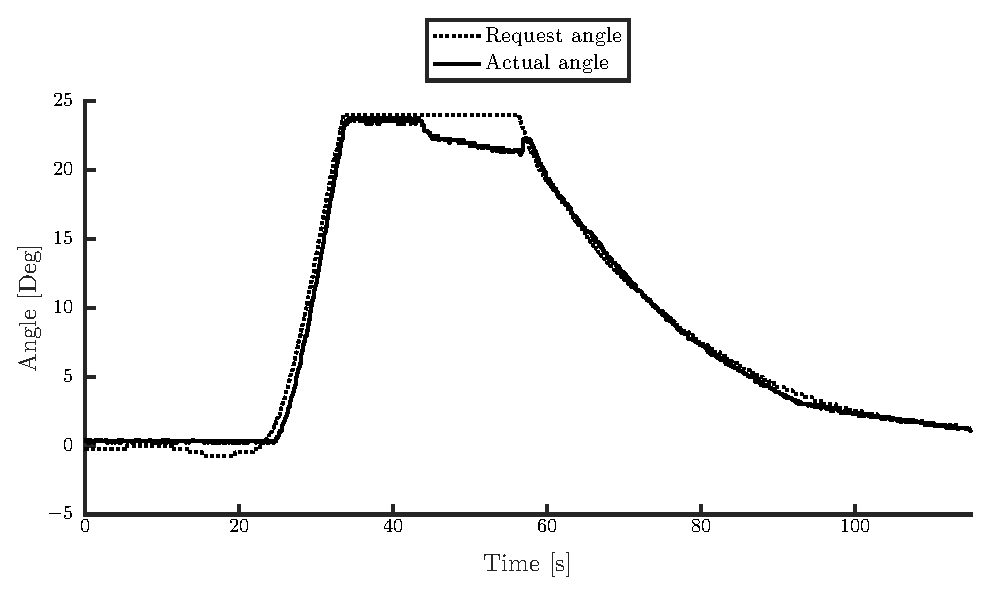
\includegraphics[width=1\linewidth]{front}
		\caption[Requested Angle and Actual Angle]{Requested Angle and Actual Angle}
		
		\label{fig:Constant_request}
	\end{figure}
	
	
	Measures to address these issues were:
	
	\begin{enumerate}
		\item A \gls{PWM} around the zero-articulation position reaching out of the dead-band was implemented for requested angles lying within this range. 
		
		\item If a constant angle is requested over a period of time, long enough to result in the described decline of the articulation, a \gls{PWM} around this value will be initiated. 
		
		\item Exactly determining the delay period made it possible to include it in the calculations for initial testing, where a feedback-loop was not present and the speed was still sufficiently low. A value of 0.26s for the front axle's reaction time and 0.30s for the back axle's respectively are too high for higher speeds.\\
		A \gls{PWM} around the desired request value was implemented in order to keep the hydraulic system active and thus eliminating some of the inertia. 
	\end{enumerate}
	
	
	
	
	
	
\end{document}